\documentclass[11pt,a4paper]{article}
\usepackage[utf8]{inputenc}
\usepackage[T1]{fontenc}
\usepackage[slovene]{babel}
\usepackage{geometry}
\usepackage{graphicx}
\usepackage{booktabs}
\usepackage{longtable}
\usepackage{pdflscape}
\usepackage{caption}
\usepackage{hyperref}
\usepackage{array}
\geometry{margin=1.8cm}
\setlength{\parindent}{0pt}
\setlength{\parskip}{0.45em}
\captionsetup{font=small, labelfont=bf}

\title{Preliminarna analiza LLM napovedi}
\author{Marjan Meglen}
\date{4. Maj 2026}

\begin{document}
\maketitle

\section{Namen in podatki}

Analiza povzema preliminarne rezultate eksperimenta \texttt{llm-trader}. Osnovna spremenljivka je $p_{yes}$, tj. verjetnost, ki jo je model pripisal razrešitvi trga v \texttt{YES}.

Podatki vsebujejo 6 trgov, 12 konfiguracij in 20 dnevnih napovedi na trg in konfiguracijo. Skupaj je analiziranih 1440 napovedi. Primerjave s parnimi t-testi so izvedene ločeno po trgih, pri čemer je par definiran z istim datumom in dvema primerjanima konfiguracijama.

\small
\setlength{\LTleft}{0pt}
\setlength{\LTright}{0pt}
\begin{longtable}{llll}
\caption{Preslikava konfiguracij.}\label{tab:configurations}\\
\toprule
Konf. & Tržne verj. & Novice & Drugi udeleženci \\
\midrule
\endfirsthead
\toprule
Konf. & Tržne verj. & Novice & Drugi udeleženci \\
\midrule
\endhead
\midrule
\multicolumn{4}{r}{Nadaljevanje na naslednji strani.} \\
\endfoot
\bottomrule
\endlastfoot
1 & da & da & llms \\
2 & da & ne & llms \\
3 & da & da & humans \\
4 & da & ne & humans \\
5 & da & da & none \\
6 & da & ne & none \\
7 & ne & da & llms \\
8 & ne & ne & llms \\
9 & ne & da & humans \\
10 & ne & ne & humans \\
11 & ne & da & none \\
12 & ne & ne & none \\
\end{longtable}
\normalsize


\section{Opisni rezultati}

\begin{figure}[htbp]
    \centering
    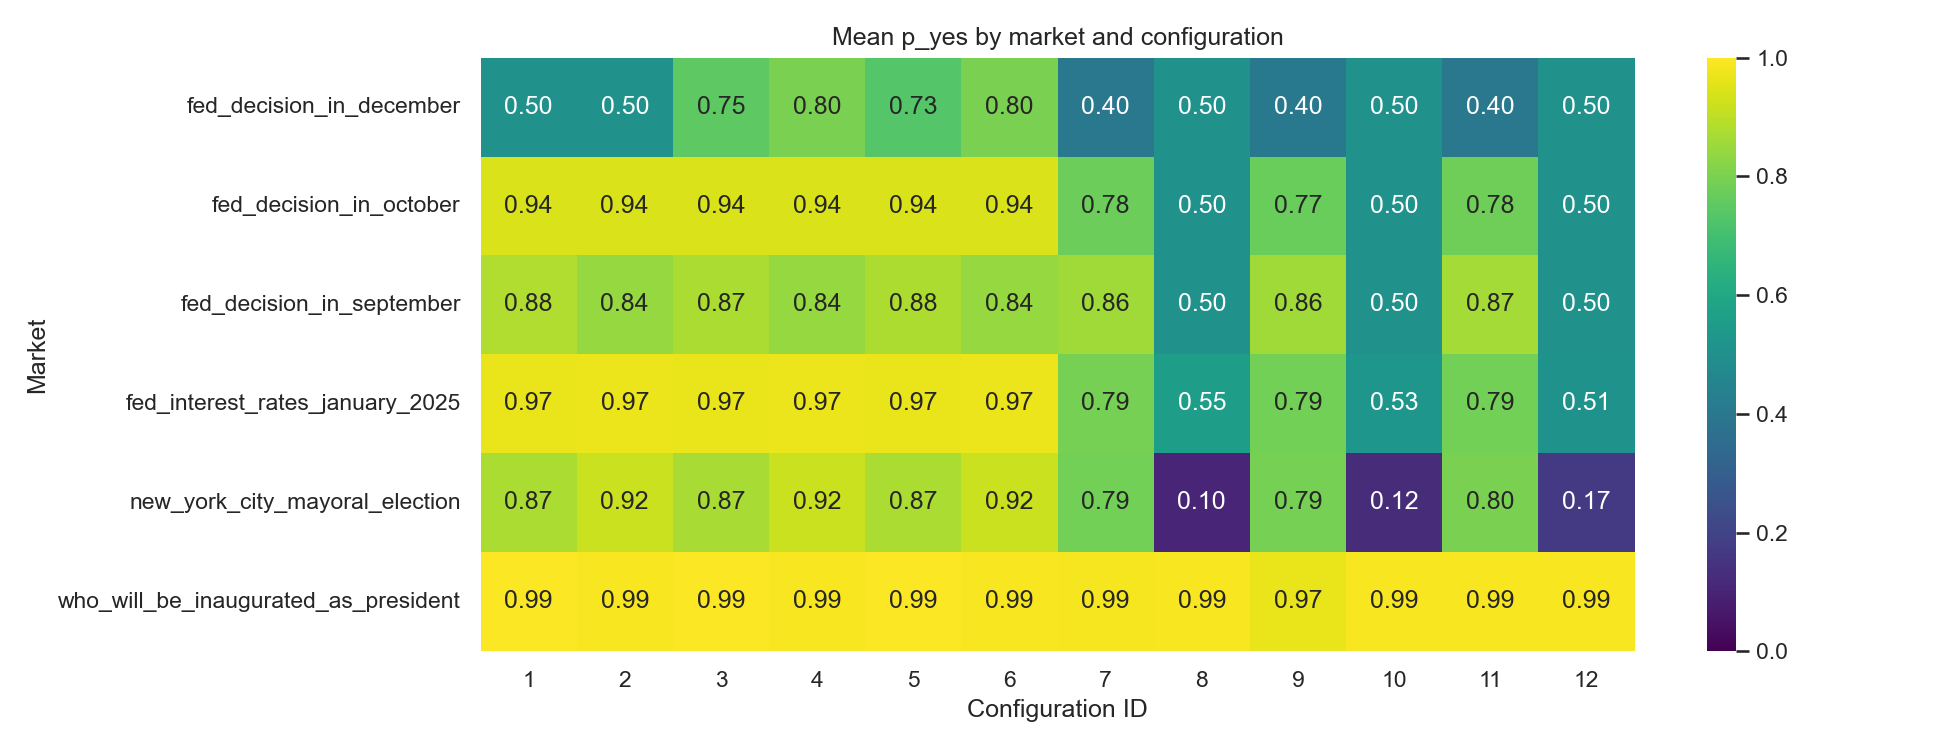
\includegraphics[width=0.95\textwidth]{../outputs/figures/heatmap_mean_p_yes_market_config.png}
    \caption{Povprečni $p_{yes}$ po trgih in konfiguracijah.}
    \label{fig:heatmap}
\end{figure}

\begin{figure}[htbp]
    \centering
    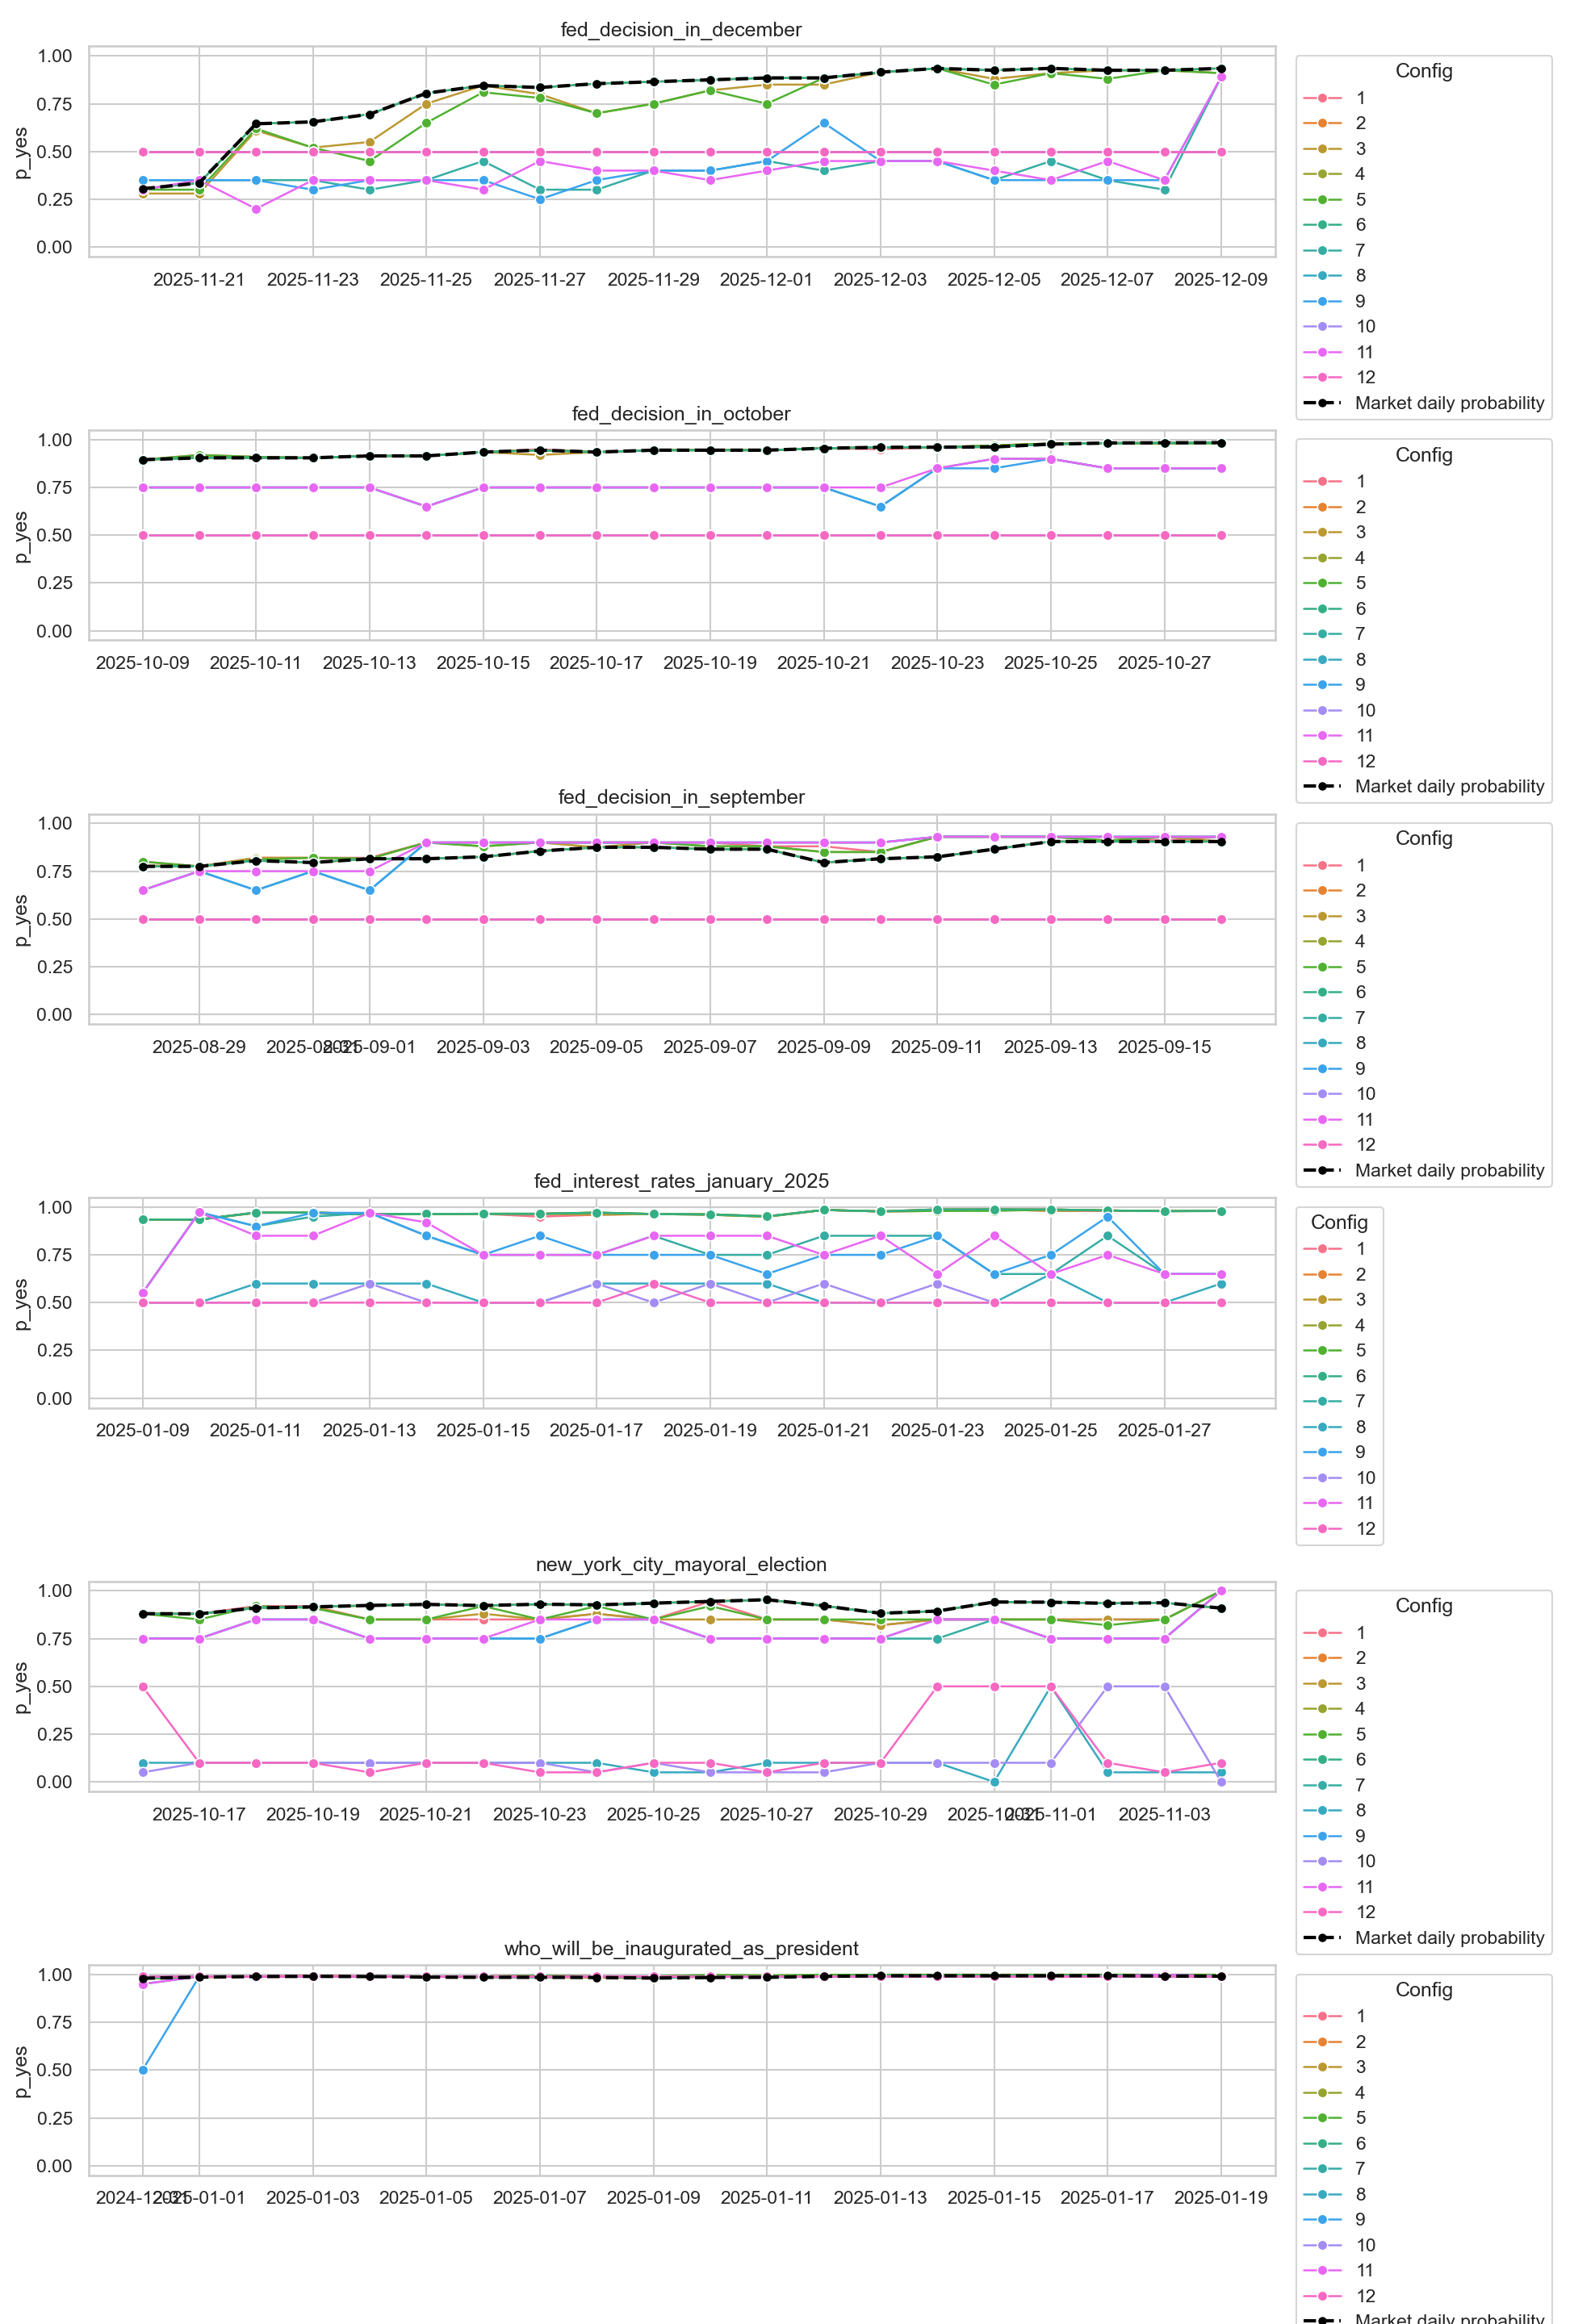
\includegraphics[width=0.98\textwidth]{../outputs/figures/lineplots_p_yes_by_market.png}
    \caption{$p_{yes}$ skozi čas po trgih in konfiguracijah.}
    \label{fig:lineplots}
\end{figure}

\begin{landscape}
\scriptsize
\setlength{\LTleft}{0pt}
\setlength{\LTright}{0pt}
\begin{longtable}{llccclrrrr}
\caption{Opisne statistike za $p_{yes}$ po trgu in konfiguraciji.}\label{tab:summary-market-config}\\
\toprule
Trg & Konf. & Tržne verj. & Novice & Udeleženci & n & M & SD & Min & Max \\
\midrule
\endfirsthead
\toprule
Trg & Konf. & Tržne verj. & Novice & Udeleženci & n & M & SD & Min & Max \\
\midrule
\endhead
\midrule
\multicolumn{10}{r}{Nadaljevanje na naslednji strani.} \\
\endfoot
\bottomrule
\endlastfoot
fed\_decision\_in\_december & 1 & da & da & llms & 20 & 0.724 & 0.192 & 0.280 & 0.910 \\
fed\_decision\_in\_december & 2 & da & ne & llms & 20 & 0.799 & 0.187 & 0.305 & 0.935 \\
fed\_decision\_in\_december & 3 & da & da & humans & 20 & 0.750 & 0.203 & 0.280 & 0.935 \\
fed\_decision\_in\_december & 4 & da & ne & humans & 20 & 0.799 & 0.187 & 0.305 & 0.935 \\
fed\_decision\_in\_december & 5 & da & da & none & 20 & 0.733 & 0.201 & 0.300 & 0.935 \\
fed\_decision\_in\_december & 6 & da & ne & none & 20 & 0.799 & 0.187 & 0.305 & 0.935 \\
fed\_decision\_in\_december & 7 & ne & da & llms & 20 & 0.400 & 0.128 & 0.300 & 0.890 \\
fed\_decision\_in\_december & 8 & ne & ne & llms & 20 & 0.500 & 0.000 & 0.500 & 0.500 \\
fed\_decision\_in\_december & 9 & ne & da & humans & 20 & 0.404 & 0.139 & 0.250 & 0.890 \\
fed\_decision\_in\_december & 10 & ne & ne & humans & 20 & 0.500 & 0.000 & 0.500 & 0.500 \\
fed\_decision\_in\_december & 11 & ne & da & none & 20 & 0.400 & 0.132 & 0.200 & 0.890 \\
fed\_decision\_in\_december & 12 & ne & ne & none & 20 & 0.500 & 0.000 & 0.500 & 0.500 \\
fed\_decision\_in\_october & 1 & da & da & llms & 20 & 0.944 & 0.027 & 0.895 & 0.985 \\
fed\_decision\_in\_october & 2 & da & ne & llms & 20 & 0.943 & 0.029 & 0.895 & 0.985 \\
fed\_decision\_in\_october & 3 & da & da & humans & 20 & 0.942 & 0.028 & 0.895 & 0.985 \\
fed\_decision\_in\_october & 4 & da & ne & humans & 20 & 0.943 & 0.029 & 0.895 & 0.985 \\
fed\_decision\_in\_october & 5 & da & da & none & 20 & 0.944 & 0.027 & 0.895 & 0.980 \\
fed\_decision\_in\_october & 6 & da & ne & none & 20 & 0.943 & 0.029 & 0.895 & 0.985 \\
fed\_decision\_in\_october & 7 & ne & da & llms & 20 & 0.775 & 0.070 & 0.650 & 0.900 \\
fed\_decision\_in\_october & 8 & ne & ne & llms & 20 & 0.500 & 0.000 & 0.500 & 0.500 \\
fed\_decision\_in\_october & 9 & ne & da & humans & 20 & 0.772 & 0.066 & 0.650 & 0.900 \\
fed\_decision\_in\_october & 10 & ne & ne & humans & 20 & 0.500 & 0.000 & 0.500 & 0.500 \\
fed\_decision\_in\_october & 11 & ne & da & none & 20 & 0.780 & 0.064 & 0.650 & 0.900 \\
fed\_decision\_in\_october & 12 & ne & ne & none & 20 & 0.500 & 0.000 & 0.500 & 0.500 \\
fed\_decision\_in\_september & 1 & da & da & llms & 20 & 0.880 & 0.049 & 0.775 & 0.930 \\
fed\_decision\_in\_september & 2 & da & ne & llms & 20 & 0.843 & 0.044 & 0.775 & 0.905 \\
fed\_decision\_in\_september & 3 & da & da & humans & 20 & 0.873 & 0.049 & 0.775 & 0.930 \\
fed\_decision\_in\_september & 4 & da & ne & humans & 20 & 0.843 & 0.044 & 0.775 & 0.905 \\
fed\_decision\_in\_september & 5 & da & da & none & 20 & 0.876 & 0.050 & 0.775 & 0.930 \\
fed\_decision\_in\_september & 6 & da & ne & none & 20 & 0.843 & 0.044 & 0.775 & 0.905 \\
fed\_decision\_in\_september & 7 & ne & da & llms & 20 & 0.856 & 0.103 & 0.650 & 0.930 \\
fed\_decision\_in\_september & 8 & ne & ne & llms & 20 & 0.500 & 0.000 & 0.500 & 0.500 \\
fed\_decision\_in\_september & 9 & ne & da & humans & 20 & 0.856 & 0.103 & 0.650 & 0.930 \\
fed\_decision\_in\_september & 10 & ne & ne & humans & 20 & 0.500 & 0.000 & 0.500 & 0.500 \\
fed\_decision\_in\_september & 11 & ne & da & none & 20 & 0.867 & 0.084 & 0.650 & 0.930 \\
fed\_decision\_in\_september & 12 & ne & ne & none & 20 & 0.500 & 0.000 & 0.500 & 0.500 \\
fed\_interest\_rates\_january\_2025 & 1 & da & da & llms & 20 & 0.967 & 0.015 & 0.935 & 0.989 \\
fed\_interest\_rates\_january\_2025 & 2 & da & ne & llms & 20 & 0.969 & 0.016 & 0.935 & 0.989 \\
fed\_interest\_rates\_january\_2025 & 3 & da & da & humans & 20 & 0.968 & 0.015 & 0.935 & 0.989 \\
fed\_interest\_rates\_january\_2025 & 4 & da & ne & humans & 20 & 0.969 & 0.016 & 0.935 & 0.989 \\
fed\_interest\_rates\_january\_2025 & 5 & da & da & none & 20 & 0.968 & 0.015 & 0.935 & 0.988 \\
fed\_interest\_rates\_january\_2025 & 6 & da & ne & none & 20 & 0.969 & 0.016 & 0.935 & 0.989 \\
fed\_interest\_rates\_january\_2025 & 7 & ne & da & llms & 20 & 0.790 & 0.119 & 0.550 & 0.973 \\
fed\_interest\_rates\_january\_2025 & 8 & ne & ne & llms & 20 & 0.552 & 0.055 & 0.500 & 0.650 \\
fed\_interest\_rates\_january\_2025 & 9 & ne & da & humans & 20 & 0.786 & 0.124 & 0.550 & 0.973 \\
fed\_interest\_rates\_january\_2025 & 10 & ne & ne & humans & 20 & 0.525 & 0.044 & 0.500 & 0.600 \\
fed\_interest\_rates\_january\_2025 & 11 & ne & da & none & 20 & 0.786 & 0.115 & 0.550 & 0.973 \\
fed\_interest\_rates\_january\_2025 & 12 & ne & ne & none & 20 & 0.505 & 0.022 & 0.500 & 0.600 \\
new\_york\_city\_mayoral\_election & 1 & da & da & llms & 20 & 0.872 & 0.043 & 0.820 & 1.000 \\
new\_york\_city\_mayoral\_election & 2 & da & ne & llms & 20 & 0.921 & 0.022 & 0.879 & 0.954 \\
new\_york\_city\_mayoral\_election & 3 & da & da & humans & 20 & 0.868 & 0.039 & 0.820 & 1.000 \\
new\_york\_city\_mayoral\_election & 4 & da & ne & humans & 20 & 0.921 & 0.022 & 0.879 & 0.954 \\
new\_york\_city\_mayoral\_election & 5 & da & da & none & 20 & 0.874 & 0.043 & 0.820 & 1.000 \\
new\_york\_city\_mayoral\_election & 6 & da & ne & none & 20 & 0.921 & 0.022 & 0.879 & 0.954 \\
new\_york\_city\_mayoral\_election & 7 & ne & da & llms & 20 & 0.787 & 0.067 & 0.750 & 1.000 \\
new\_york\_city\_mayoral\_election & 8 & ne & ne & llms & 20 & 0.102 & 0.098 & 0.000 & 0.500 \\
new\_york\_city\_mayoral\_election & 9 & ne & da & humans & 20 & 0.792 & 0.067 & 0.750 & 1.000 \\
new\_york\_city\_mayoral\_election & 10 & ne & ne & humans & 20 & 0.122 & 0.132 & 0.000 & 0.500 \\
new\_york\_city\_mayoral\_election & 11 & ne & da & none & 20 & 0.797 & 0.068 & 0.750 & 1.000 \\
new\_york\_city\_mayoral\_election & 12 & ne & ne & none & 20 & 0.168 & 0.172 & 0.050 & 0.500 \\
who\_will\_be\_inaugurated\_as\_president & 1 & da & da & llms & 20 & 0.994 & 0.005 & 0.981 & 0.999 \\
who\_will\_be\_inaugurated\_as\_president & 2 & da & ne & llms & 20 & 0.989 & 0.004 & 0.980 & 0.995 \\
who\_will\_be\_inaugurated\_as\_president & 3 & da & da & humans & 20 & 0.993 & 0.005 & 0.980 & 0.999 \\
who\_will\_be\_inaugurated\_as\_president & 4 & da & ne & humans & 20 & 0.990 & 0.004 & 0.980 & 0.995 \\
who\_will\_be\_inaugurated\_as\_president & 5 & da & da & none & 20 & 0.994 & 0.006 & 0.981 & 0.999 \\
who\_will\_be\_inaugurated\_as\_president & 6 & da & ne & none & 20 & 0.990 & 0.004 & 0.981 & 0.995 \\
who\_will\_be\_inaugurated\_as\_president & 7 & ne & da & llms & 20 & 0.988 & 0.009 & 0.950 & 0.990 \\
who\_will\_be\_inaugurated\_as\_president & 8 & ne & ne & llms & 20 & 0.990 & 0.000 & 0.990 & 0.990 \\
who\_will\_be\_inaugurated\_as\_president & 9 & ne & da & humans & 20 & 0.966 & 0.110 & 0.500 & 1.000 \\
who\_will\_be\_inaugurated\_as\_president & 10 & ne & ne & humans & 20 & 0.990 & 0.000 & 0.990 & 0.990 \\
who\_will\_be\_inaugurated\_as\_president & 11 & ne & da & none & 20 & 0.989 & 0.009 & 0.950 & 1.000 \\
who\_will\_be\_inaugurated\_as\_president & 12 & ne & ne & none & 20 & 0.990 & 0.000 & 0.990 & 0.990 \\
\end{longtable}
\normalsize

\end{landscape}

\begin{landscape}
\scriptsize
\setlength{\LTleft}{0pt}
\setlength{\LTright}{0pt}
\begin{longtable}{lllrrr}
\caption{Opisne statistike za $p_{yes}$ po trgu in posameznem faktorju.}\label{tab:summary-market-factor}\\
\toprule
Trg & Faktor & Nivo & n & M & SD \\
\midrule
\endfirsthead
\toprule
Trg & Faktor & Nivo & n & M & SD \\
\midrule
\endhead
\midrule
\multicolumn{6}{r}{Nadaljevanje na naslednji strani.} \\
\endfoot
\bottomrule
\endlastfoot
fed\_decision\_in\_december & tržne verjetnosti & ne & 120 & 0.451 & 0.105 \\
fed\_decision\_in\_december & tržne verjetnosti & da & 120 & 0.767 & 0.192 \\
fed\_decision\_in\_october & tržne verjetnosti & ne & 120 & 0.638 & 0.146 \\
fed\_decision\_in\_october & tržne verjetnosti & da & 120 & 0.943 & 0.028 \\
fed\_decision\_in\_september & tržne verjetnosti & ne & 120 & 0.680 & 0.193 \\
fed\_decision\_in\_september & tržne verjetnosti & da & 120 & 0.860 & 0.049 \\
fed\_interest\_rates\_january\_2025 & tržne verjetnosti & ne & 120 & 0.657 & 0.158 \\
fed\_interest\_rates\_january\_2025 & tržne verjetnosti & da & 120 & 0.969 & 0.015 \\
new\_york\_city\_mayoral\_election & tržne verjetnosti & ne & 120 & 0.462 & 0.349 \\
new\_york\_city\_mayoral\_election & tržne verjetnosti & da & 120 & 0.896 & 0.041 \\
who\_will\_be\_inaugurated\_as\_president & tržne verjetnosti & ne & 120 & 0.985 & 0.045 \\
who\_will\_be\_inaugurated\_as\_president & tržne verjetnosti & da & 120 & 0.992 & 0.005 \\
fed\_decision\_in\_december & novice & ne & 120 & 0.649 & 0.198 \\
fed\_decision\_in\_december & novice & da & 120 & 0.568 & 0.236 \\
fed\_decision\_in\_october & novice & ne & 120 & 0.721 & 0.223 \\
fed\_decision\_in\_october & novice & da & 120 & 0.860 & 0.098 \\
fed\_decision\_in\_september & novice & ne & 120 & 0.671 & 0.175 \\
fed\_decision\_in\_september & novice & da & 120 & 0.868 & 0.076 \\
fed\_interest\_rates\_january\_2025 & novice & ne & 120 & 0.748 & 0.225 \\
fed\_interest\_rates\_january\_2025 & novice & da & 120 & 0.877 & 0.123 \\
new\_york\_city\_mayoral\_election & novice & ne & 120 & 0.526 & 0.409 \\
new\_york\_city\_mayoral\_election & novice & da & 120 & 0.832 & 0.068 \\
who\_will\_be\_inaugurated\_as\_president & novice & ne & 120 & 0.990 & 0.003 \\
who\_will\_be\_inaugurated\_as\_president & novice & da & 120 & 0.987 & 0.045 \\
fed\_decision\_in\_december & drugi udeleženci & humans & 80 & 0.613 & 0.225 \\
fed\_decision\_in\_december & drugi udeleženci & llms & 80 & 0.606 & 0.218 \\
fed\_decision\_in\_december & drugi udeleženci & none & 80 & 0.608 & 0.222 \\
fed\_decision\_in\_october & drugi udeleženci & humans & 80 & 0.789 & 0.186 \\
fed\_decision\_in\_october & drugi udeleženci & llms & 80 & 0.790 & 0.186 \\
fed\_decision\_in\_october & drugi udeleženci & none & 80 & 0.792 & 0.186 \\
fed\_decision\_in\_september & drugi udeleženci & humans & 80 & 0.768 & 0.167 \\
fed\_decision\_in\_september & drugi udeleženci & llms & 80 & 0.770 & 0.168 \\
fed\_decision\_in\_september & drugi udeleženci & none & 80 & 0.771 & 0.167 \\
fed\_interest\_rates\_january\_2025 & drugi udeleženci & humans & 80 & 0.812 & 0.194 \\
fed\_interest\_rates\_january\_2025 & drugi udeleženci & llms & 80 & 0.820 & 0.184 \\
fed\_interest\_rates\_january\_2025 & drugi udeleženci & none & 80 & 0.807 & 0.200 \\
new\_york\_city\_mayoral\_election & drugi udeleženci & humans & 80 & 0.676 & 0.334 \\
new\_york\_city\_mayoral\_election & drugi udeleženci & llms & 80 & 0.671 & 0.339 \\
new\_york\_city\_mayoral\_election & drugi udeleženci & none & 80 & 0.690 & 0.321 \\
who\_will\_be\_inaugurated\_as\_president & drugi udeleženci & humans & 80 & 0.985 & 0.055 \\
who\_will\_be\_inaugurated\_as\_president & drugi udeleženci & llms & 80 & 0.990 & 0.006 \\
who\_will\_be\_inaugurated\_as\_president & drugi udeleženci & none & 80 & 0.990 & 0.006 \\
\end{longtable}
\normalsize

\end{landscape}

\section{Parni t-testi}

Pozitivna razlika pomeni, da je bila vrednost $p_{yes}$ višja v konfiguraciji A kot v konfiguraciji B. V tabelah so prikazani povprečna razlika, 95\% interval zaupanja, statistika $t$ in vrednost $p$.

\subsection{Učinek novic}

\begin{landscape}
\scriptsize
\setlength{\LTleft}{0pt}
\setlength{\LTright}{0pt}
\begin{longtable}{llrrrrrrrr}
\caption{Parni t-testi za učinek novic po trgih.}\label{tab:ttests-news}\\
\toprule
Trg & Primerjava & A & B & n & $M_\Delta$ & CI spod. & CI zg. & t & p \\
\midrule
\endfirsthead
\toprule
Trg & Primerjava & A & B & n & $M_\Delta$ & CI spod. & CI zg. & t & p \\
\midrule
\endhead
\midrule
\multicolumn{10}{r}{Nadaljevanje na naslednji strani.} \\
\endfoot
\bottomrule
\endlastfoot
fed\_decision\_in\_december & news\_shown\_minus\_hidden & 1 & 2 & 20 & -0.075 & -0.104 & -0.046 & -5.479 & 2.76e-05 \\
fed\_decision\_in\_october & news\_shown\_minus\_hidden & 1 & 2 & 20 & 1.00e-03 & -0.001 & 0.003 & 0.919 & 0.370 \\
fed\_decision\_in\_september & news\_shown\_minus\_hidden & 1 & 2 & 20 & 0.037 & 0.023 & 0.051 & 5.582 & 2.21e-05 \\
fed\_interest\_rates\_january\_2025 & news\_shown\_minus\_hidden & 1 & 2 & 20 & -0.003 & -0.005 & -4.63e-04 & -2.569 & 0.019 \\
new\_york\_city\_mayoral\_election & news\_shown\_minus\_hidden & 1 & 2 & 20 & -0.048 & -0.072 & -0.025 & -4.341 & 3.52e-04 \\
who\_will\_be\_inaugurated\_as\_president & news\_shown\_minus\_hidden & 1 & 2 & 20 & 0.005 & 0.003 & 0.006 & 7.635 & 3.33e-07 \\
fed\_decision\_in\_december & news\_shown\_minus\_hidden & 3 & 4 & 20 & -0.049 & -0.072 & -0.026 & -4.391 & 3.14e-04 \\
fed\_decision\_in\_october & news\_shown\_minus\_hidden & 3 & 4 & 20 & -5.00e-04 & -0.003 & 0.002 & -0.352 & 0.728 \\
fed\_decision\_in\_september & news\_shown\_minus\_hidden & 3 & 4 & 20 & 0.030 & 0.016 & 0.044 & 4.485 & 2.54e-04 \\
fed\_interest\_rates\_january\_2025 & news\_shown\_minus\_hidden & 3 & 4 & 20 & -0.002 & -0.003 & -7.10e-05 & -2.190 & 0.041 \\
new\_york\_city\_mayoral\_election & news\_shown\_minus\_hidden & 3 & 4 & 20 & -0.052 & -0.075 & -0.030 & -4.832 & 1.16e-04 \\
who\_will\_be\_inaugurated\_as\_president & news\_shown\_minus\_hidden & 3 & 4 & 20 & 0.003 & 0.002 & 0.005 & 4.419 & 2.95e-04 \\
fed\_decision\_in\_december & news\_shown\_minus\_hidden & 5 & 6 & 20 & -0.066 & -0.098 & -0.034 & -4.320 & 3.69e-04 \\
fed\_decision\_in\_october & news\_shown\_minus\_hidden & 5 & 6 & 20 & 0.001 & -9.67e-04 & 0.003 & 1.077 & 0.295 \\
fed\_decision\_in\_september & news\_shown\_minus\_hidden & 5 & 6 & 20 & 0.033 & 0.020 & 0.046 & 5.275 & 4.31e-05 \\
fed\_interest\_rates\_january\_2025 & news\_shown\_minus\_hidden & 5 & 6 & 20 & -0.001 & -0.003 & -7.02e-05 & -2.212 & 0.039 \\
new\_york\_city\_mayoral\_election & news\_shown\_minus\_hidden & 5 & 6 & 20 & -0.046 & -0.070 & -0.022 & -4.079 & 6.40e-04 \\
who\_will\_be\_inaugurated\_as\_president & news\_shown\_minus\_hidden & 5 & 6 & 20 & 0.004 & 0.003 & 0.006 & 4.897 & 1.00e-04 \\
fed\_decision\_in\_december & news\_shown\_minus\_hidden & 7 & 8 & 20 & -0.100 & -0.160 & -0.041 & -3.518 & 0.002 \\
fed\_decision\_in\_october & news\_shown\_minus\_hidden & 7 & 8 & 20 & 0.275 & 0.242 & 0.308 & 17.626 & 3.12e-13 \\
fed\_decision\_in\_september & news\_shown\_minus\_hidden & 7 & 8 & 20 & 0.356 & 0.308 & 0.405 & 15.537 & 2.96e-12 \\
fed\_interest\_rates\_january\_2025 & news\_shown\_minus\_hidden & 7 & 8 & 20 & 0.237 & 0.178 & 0.297 & 8.359 & 8.67e-08 \\
new\_york\_city\_mayoral\_election & news\_shown\_minus\_hidden & 7 & 8 & 20 & 0.685 & 0.624 & 0.746 & 23.405 & 1.80e-15 \\
who\_will\_be\_inaugurated\_as\_president & news\_shown\_minus\_hidden & 7 & 8 & 20 & -0.002 & -0.006 & 0.002 & -1.000 & 0.330 \\
fed\_decision\_in\_december & news\_shown\_minus\_hidden & 9 & 10 & 20 & -0.095 & -0.161 & -0.030 & -3.062 & 0.006 \\
fed\_decision\_in\_october & news\_shown\_minus\_hidden & 9 & 10 & 20 & 0.272 & 0.242 & 0.303 & 18.508 & 1.30e-13 \\
fed\_decision\_in\_september & news\_shown\_minus\_hidden & 9 & 10 & 20 & 0.356 & 0.308 & 0.405 & 15.537 & 2.96e-12 \\
fed\_interest\_rates\_january\_2025 & news\_shown\_minus\_hidden & 9 & 10 & 20 & 0.261 & 0.202 & 0.320 & 9.234 & 1.87e-08 \\
new\_york\_city\_mayoral\_election & news\_shown\_minus\_hidden & 9 & 10 & 20 & 0.670 & 0.593 & 0.747 & 18.164 & 1.82e-13 \\
who\_will\_be\_inaugurated\_as\_president & news\_shown\_minus\_hidden & 9 & 10 & 20 & -0.024 & -0.075 & 0.027 & -0.978 & 0.340 \\
fed\_decision\_in\_december & news\_shown\_minus\_hidden & 11 & 12 & 20 & -0.100 & -0.162 & -0.039 & -3.410 & 0.003 \\
fed\_decision\_in\_october & news\_shown\_minus\_hidden & 11 & 12 & 20 & 0.280 & 0.250 & 0.310 & 19.670 & 4.31e-14 \\
fed\_decision\_in\_september & news\_shown\_minus\_hidden & 11 & 12 & 20 & 0.366 & 0.327 & 0.406 & 19.412 & 5.48e-14 \\
fed\_interest\_rates\_january\_2025 & news\_shown\_minus\_hidden & 11 & 12 & 20 & 0.281 & 0.227 & 0.334 & 10.980 & 1.14e-09 \\
new\_york\_city\_mayoral\_election & news\_shown\_minus\_hidden & 11 & 12 & 20 & 0.630 & 0.544 & 0.716 & 15.387 & 3.51e-12 \\
who\_will\_be\_inaugurated\_as\_president & news\_shown\_minus\_hidden & 11 & 12 & 20 & -0.002 & -0.006 & 0.003 & -0.719 & 0.481 \\
\end{longtable}
\normalsize

\end{landscape}

\subsection{Učinek prikaza tržnih verjetnosti}

\begin{landscape}
\scriptsize
\setlength{\LTleft}{0pt}
\setlength{\LTright}{0pt}
\begin{longtable}{llrrrrrrrr}
\caption{Parni t-testi za učinek prikaza tržnih verjetnosti po trgih.}\label{tab:ttests-market-prob}\\
\toprule
Trg & Primerjava & A & B & n & $M_\Delta$ & CI spod. & CI zg. & t & p \\
\midrule
\endfirsthead
\toprule
Trg & Primerjava & A & B & n & $M_\Delta$ & CI spod. & CI zg. & t & p \\
\midrule
\endhead
\midrule
\multicolumn{10}{r}{Nadaljevanje na naslednji strani.} \\
\endfoot
\bottomrule
\endlastfoot
fed\_decision\_in\_december & market\_probs\_shown\_minus\_hidden & 1 & 7 & 20 & 0.325 & 0.236 & 0.413 & 7.693 & 2.98e-07 \\
fed\_decision\_in\_october & market\_probs\_shown\_minus\_hidden & 1 & 7 & 20 & 0.169 & 0.143 & 0.194 & 13.719 & 2.62e-11 \\
fed\_decision\_in\_september & market\_probs\_shown\_minus\_hidden & 1 & 7 & 20 & 0.024 & -0.006 & 0.054 & 1.655 & 0.114 \\
fed\_interest\_rates\_january\_2025 & market\_probs\_shown\_minus\_hidden & 1 & 7 & 20 & 0.177 & 0.121 & 0.234 & 6.580 & 2.68e-06 \\
new\_york\_city\_mayoral\_election & market\_probs\_shown\_minus\_hidden & 1 & 7 & 20 & 0.085 & 0.062 & 0.107 & 7.904 & 2.00e-07 \\
who\_will\_be\_inaugurated\_as\_president & market\_probs\_shown\_minus\_hidden & 1 & 7 & 20 & 0.006 & 0.003 & 0.009 & 3.808 & 0.001 \\
fed\_decision\_in\_december & market\_probs\_shown\_minus\_hidden & 2 & 8 & 20 & 0.299 & 0.212 & 0.386 & 7.160 & 8.36e-07 \\
fed\_decision\_in\_october & market\_probs\_shown\_minus\_hidden & 2 & 8 & 20 & 0.443 & 0.429 & 0.456 & 69.339 & 2.58e-24 \\
fed\_decision\_in\_september & market\_probs\_shown\_minus\_hidden & 2 & 8 & 20 & 0.343 & 0.322 & 0.364 & 34.611 & 1.25e-18 \\
fed\_interest\_rates\_january\_2025 & market\_probs\_shown\_minus\_hidden & 2 & 8 & 20 & 0.417 & 0.390 & 0.444 & 32.789 & 3.45e-18 \\
new\_york\_city\_mayoral\_election & market\_probs\_shown\_minus\_hidden & 2 & 8 & 20 & 0.818 & 0.772 & 0.864 & 37.020 & 3.55e-19 \\
who\_will\_be\_inaugurated\_as\_president & market\_probs\_shown\_minus\_hidden & 2 & 8 & 20 & -7.00e-04 & -0.003 & 0.001 & -0.761 & 0.456 \\
fed\_decision\_in\_december & market\_probs\_shown\_minus\_hidden & 3 & 9 & 20 & 0.346 & 0.249 & 0.442 & 7.482 & 4.46e-07 \\
fed\_decision\_in\_october & market\_probs\_shown\_minus\_hidden & 3 & 9 & 20 & 0.170 & 0.145 & 0.194 & 14.522 & 9.72e-12 \\
fed\_decision\_in\_september & market\_probs\_shown\_minus\_hidden & 3 & 9 & 20 & 0.016 & -0.014 & 0.047 & 1.130 & 0.272 \\
fed\_interest\_rates\_january\_2025 & market\_probs\_shown\_minus\_hidden & 3 & 9 & 20 & 0.182 & 0.124 & 0.241 & 6.515 & 3.06e-06 \\
new\_york\_city\_mayoral\_election & market\_probs\_shown\_minus\_hidden & 3 & 9 & 20 & 0.076 & 0.054 & 0.097 & 7.431 & 4.93e-07 \\
who\_will\_be\_inaugurated\_as\_president & market\_probs\_shown\_minus\_hidden & 3 & 9 & 20 & 0.027 & -0.023 & 0.077 & 1.142 & 0.268 \\
fed\_decision\_in\_december & market\_probs\_shown\_minus\_hidden & 4 & 10 & 20 & 0.299 & 0.212 & 0.386 & 7.160 & 8.36e-07 \\
fed\_decision\_in\_october & market\_probs\_shown\_minus\_hidden & 4 & 10 & 20 & 0.443 & 0.429 & 0.456 & 69.339 & 2.58e-24 \\
fed\_decision\_in\_september & market\_probs\_shown\_minus\_hidden & 4 & 10 & 20 & 0.343 & 0.322 & 0.364 & 34.611 & 1.25e-18 \\
fed\_interest\_rates\_january\_2025 & market\_probs\_shown\_minus\_hidden & 4 & 10 & 20 & 0.444 & 0.424 & 0.465 & 44.814 & 9.80e-21 \\
new\_york\_city\_mayoral\_election & market\_probs\_shown\_minus\_hidden & 4 & 10 & 20 & 0.798 & 0.738 & 0.859 & 27.634 & 8.34e-17 \\
who\_will\_be\_inaugurated\_as\_president & market\_probs\_shown\_minus\_hidden & 4 & 10 & 20 & -1.00e-04 & -0.002 & 0.002 & -0.117 & 0.908 \\
fed\_decision\_in\_december & market\_probs\_shown\_minus\_hidden & 5 & 11 & 20 & 0.334 & 0.245 & 0.422 & 7.878 & 2.10e-07 \\
fed\_decision\_in\_october & market\_probs\_shown\_minus\_hidden & 5 & 11 & 20 & 0.164 & 0.142 & 0.186 & 15.670 & 2.54e-12 \\
fed\_decision\_in\_september & market\_probs\_shown\_minus\_hidden & 5 & 11 & 20 & 0.009 & -0.012 & 0.031 & 0.919 & 0.370 \\
fed\_interest\_rates\_january\_2025 & market\_probs\_shown\_minus\_hidden & 5 & 11 & 20 & 0.182 & 0.126 & 0.239 & 6.796 & 1.73e-06 \\
new\_york\_city\_mayoral\_election & market\_probs\_shown\_minus\_hidden & 5 & 11 & 20 & 0.077 & 0.052 & 0.102 & 6.434 & 3.61e-06 \\
who\_will\_be\_inaugurated\_as\_president & market\_probs\_shown\_minus\_hidden & 5 & 11 & 20 & 0.005 & 0.002 & 0.009 & 3.236 & 0.004 \\
fed\_decision\_in\_december & market\_probs\_shown\_minus\_hidden & 6 & 12 & 20 & 0.299 & 0.212 & 0.386 & 7.160 & 8.36e-07 \\
fed\_decision\_in\_october & market\_probs\_shown\_minus\_hidden & 6 & 12 & 20 & 0.443 & 0.429 & 0.456 & 69.339 & 2.58e-24 \\
fed\_decision\_in\_september & market\_probs\_shown\_minus\_hidden & 6 & 12 & 20 & 0.343 & 0.322 & 0.364 & 34.611 & 1.25e-18 \\
fed\_interest\_rates\_january\_2025 & market\_probs\_shown\_minus\_hidden & 6 & 12 & 20 & 0.464 & 0.451 & 0.478 & 73.554 & 8.43e-25 \\
new\_york\_city\_mayoral\_election & market\_probs\_shown\_minus\_hidden & 6 & 12 & 20 & 0.753 & 0.670 & 0.836 & 18.983 & 8.21e-14 \\
who\_will\_be\_inaugurated\_as\_president & market\_probs\_shown\_minus\_hidden & 6 & 12 & 20 & -5.00e-04 & -0.002 & 0.001 & -0.568 & 0.576 \\
\end{longtable}
\normalsize

\end{landscape}

\subsection{Učinek informacije o drugih udeležencih}

\begin{landscape}
\scriptsize
\setlength{\LTleft}{0pt}
\setlength{\LTright}{0pt}
\begin{longtable}{llrrrrrrrr}
\caption{Parni t-testi za učinek informacije o drugih udeležencih po trgih.}\label{tab:ttests-trader}\\
\toprule
Trg & Primerjava & A & B & n & $M_\Delta$ & CI spod. & CI zg. & t & p \\
\midrule
\endfirsthead
\toprule
Trg & Primerjava & A & B & n & $M_\Delta$ & CI spod. & CI zg. & t & p \\
\midrule
\endhead
\midrule
\multicolumn{10}{r}{Nadaljevanje na naslednji strani.} \\
\endfoot
\bottomrule
\endlastfoot
fed\_decision\_in\_december & llms - humans; tržne verj.=da, novice=da & 1 & 3 & 20 & -0.026 & -0.050 & -0.002 & -2.311 & 0.032 \\
fed\_decision\_in\_october & llms - humans; tržne verj.=da, novice=da & 1 & 3 & 20 & 0.001 & -0.002 & 0.005 & 0.900 & 0.379 \\
fed\_decision\_in\_september & llms - humans; tržne verj.=da, novice=da & 1 & 3 & 20 & 0.007 & 0.001 & 0.013 & 2.529 & 0.020 \\
fed\_interest\_rates\_january\_2025 & llms - humans; tržne verj.=da, novice=da & 1 & 3 & 20 & -9.00e-04 & -0.002 & 6.75e-04 & -1.196 & 0.247 \\
new\_york\_city\_mayoral\_election & llms - humans; tržne verj.=da, novice=da & 1 & 3 & 20 & 0.004 & -0.007 & 0.014 & 0.779 & 0.445 \\
who\_will\_be\_inaugurated\_as\_president & llms - humans; tržne verj.=da, novice=da & 1 & 3 & 20 & 7.00e-04 & -7.94e-05 & 0.001 & 1.880 & 0.076 \\
fed\_decision\_in\_december & llms - none; tržne verj.=da, novice=da & 1 & 5 & 20 & -0.009 & -0.033 & 0.015 & -0.792 & 0.438 \\
fed\_decision\_in\_october & llms - none; tržne verj.=da, novice=da & 1 & 5 & 20 & -2.50e-05 & -0.001 & 0.001 & -0.040 & 0.968 \\
fed\_decision\_in\_september & llms - none; tržne verj.=da, novice=da & 1 & 5 & 20 & 0.004 & -8.59e-04 & 0.009 & 1.741 & 0.098 \\
fed\_interest\_rates\_january\_2025 & llms - none; tržne verj.=da, novice=da & 1 & 5 & 20 & -0.001 & -0.004 & 0.001 & -1.076 & 0.295 \\
new\_york\_city\_mayoral\_election & llms - none; tržne verj.=da, novice=da & 1 & 5 & 20 & -0.002 & -0.013 & 0.008 & -0.448 & 0.659 \\
who\_will\_be\_inaugurated\_as\_president & llms - none; tržne verj.=da, novice=da & 1 & 5 & 20 & 2.50e-05 & -8.68e-04 & 9.18e-04 & 0.059 & 0.954 \\
fed\_decision\_in\_december & humans - none; tržne verj.=da, novice=da & 3 & 5 & 20 & 0.017 & -0.002 & 0.036 & 1.918 & 0.070 \\
fed\_decision\_in\_october & humans - none; tržne verj.=da, novice=da & 3 & 5 & 20 & -0.002 & -0.004 & 0.001 & -1.125 & 0.275 \\
fed\_decision\_in\_september & humans - none; tržne verj.=da, novice=da & 3 & 5 & 20 & -0.003 & -0.007 & 0.001 & -1.476 & 0.156 \\
fed\_interest\_rates\_january\_2025 & humans - none; tržne verj.=da, novice=da & 3 & 5 & 20 & -3.00e-04 & -0.002 & 0.001 & -0.357 & 0.725 \\
new\_york\_city\_mayoral\_election & humans - none; tržne verj.=da, novice=da & 3 & 5 & 20 & -0.006 & -0.017 & 0.005 & -1.199 & 0.245 \\
who\_will\_be\_inaugurated\_as\_president & humans - none; tržne verj.=da, novice=da & 3 & 5 & 20 & -6.75e-04 & -0.001 & 6.99e-05 & -1.897 & 0.073 \\
fed\_decision\_in\_december & llms - humans; tržne verj.=da, novice=ne & 2 & 4 & 20 & 0.000 & 0.000 & 0.000 & 0.000 & 1.000 \\
fed\_decision\_in\_october & llms - humans; tržne verj.=da, novice=ne & 2 & 4 & 20 & 0.000 & 0.000 & 0.000 & 0.000 & 1.000 \\
fed\_decision\_in\_september & llms - humans; tržne verj.=da, novice=ne & 2 & 4 & 20 & 0.000 & 0.000 & 0.000 & 0.000 & 1.000 \\
fed\_interest\_rates\_january\_2025 & llms - humans; tržne verj.=da, novice=ne & 2 & 4 & 20 & 0.000 & 0.000 & 0.000 & 0.000 & 1.000 \\
new\_york\_city\_mayoral\_election & llms - humans; tržne verj.=da, novice=ne & 2 & 4 & 20 & -2.50e-05 & -7.73e-05 & 2.73e-05 & -1.000 & 0.330 \\
who\_will\_be\_inaugurated\_as\_president & llms - humans; tržne verj.=da, novice=ne & 2 & 4 & 20 & -6.00e-04 & -0.001 & 1.27e-04 & -1.728 & 0.100 \\
fed\_decision\_in\_december & llms - none; tržne verj.=da, novice=ne & 2 & 6 & 20 & 0.000 & 0.000 & 0.000 & 0.000 & 1.000 \\
fed\_decision\_in\_october & llms - none; tržne verj.=da, novice=ne & 2 & 6 & 20 & 0.000 & 0.000 & 0.000 & 0.000 & 1.000 \\
fed\_decision\_in\_september & llms - none; tržne verj.=da, novice=ne & 2 & 6 & 20 & 0.000 & 0.000 & 0.000 & 0.000 & 1.000 \\
fed\_interest\_rates\_january\_2025 & llms - none; tržne verj.=da, novice=ne & 2 & 6 & 20 & 0.000 & 0.000 & 0.000 & 0.000 & 1.000 \\
new\_york\_city\_mayoral\_election & llms - none; tržne verj.=da, novice=ne & 2 & 6 & 20 & -2.50e-05 & -7.73e-05 & 2.73e-05 & -1.000 & 0.330 \\
who\_will\_be\_inaugurated\_as\_president & llms - none; tržne verj.=da, novice=ne & 2 & 6 & 20 & -2.00e-04 & -0.001 & 6.50e-04 & -0.492 & 0.628 \\
fed\_decision\_in\_december & humans - none; tržne verj.=da, novice=ne & 4 & 6 & 20 & 0.000 & 0.000 & 0.000 & 0.000 & 1.000 \\
fed\_decision\_in\_october & humans - none; tržne verj.=da, novice=ne & 4 & 6 & 20 & 0.000 & 0.000 & 0.000 & 0.000 & 1.000 \\
fed\_decision\_in\_september & humans - none; tržne verj.=da, novice=ne & 4 & 6 & 20 & 0.000 & 0.000 & 0.000 & 0.000 & 1.000 \\
fed\_interest\_rates\_january\_2025 & humans - none; tržne verj.=da, novice=ne & 4 & 6 & 20 & 0.000 & 0.000 & 0.000 & 0.000 & 1.000 \\
new\_york\_city\_mayoral\_election & humans - none; tržne verj.=da, novice=ne & 4 & 6 & 20 & 0.000 & 0.000 & 0.000 & 0.000 & 1.000 \\
who\_will\_be\_inaugurated\_as\_president & humans - none; tržne verj.=da, novice=ne & 4 & 6 & 20 & 4.00e-04 & -6.09e-04 & 0.001 & 0.830 & 0.417 \\
fed\_decision\_in\_december & llms - humans; tržne verj.=ne, novice=da & 7 & 9 & 20 & -0.005 & -0.038 & 0.028 & -0.317 & 0.755 \\
fed\_decision\_in\_october & llms - humans; tržne verj.=ne, novice=da & 7 & 9 & 20 & 0.003 & -0.003 & 0.008 & 1.000 & 0.330 \\
fed\_decision\_in\_september & llms - humans; tržne verj.=ne, novice=da & 7 & 9 & 20 & 0.000 & 0.000 & 0.000 & 0.000 & 1.000 \\
fed\_interest\_rates\_january\_2025 & llms - humans; tržne verj.=ne, novice=da & 7 & 9 & 20 & 0.004 & -0.024 & 0.032 & 0.295 & 0.772 \\
new\_york\_city\_mayoral\_election & llms - humans; tržne verj.=ne, novice=da & 7 & 9 & 20 & -0.005 & -0.015 & 0.005 & -1.000 & 0.330 \\
who\_will\_be\_inaugurated\_as\_president & llms - humans; tržne verj.=ne, novice=da & 7 & 9 & 20 & 0.022 & -0.025 & 0.069 & 0.976 & 0.341 \\
fed\_decision\_in\_december & llms - none; tržne verj.=ne, novice=da & 7 & 11 & 20 & -2.78e-18 & -0.036 & 0.036 & -1.60e-16 & 1.000 \\
fed\_decision\_in\_october & llms - none; tržne verj.=ne, novice=da & 7 & 11 & 20 & -0.005 & -0.015 & 0.005 & -1.000 & 0.330 \\
fed\_decision\_in\_september & llms - none; tržne verj.=ne, novice=da & 7 & 11 & 20 & -0.010 & -0.024 & 0.004 & -1.453 & 0.163 \\
fed\_interest\_rates\_january\_2025 & llms - none; tržne verj.=ne, novice=da & 7 & 11 & 20 & 0.004 & -0.036 & 0.044 & 0.211 & 0.835 \\
new\_york\_city\_mayoral\_election & llms - none; tržne verj.=ne, novice=da & 7 & 11 & 20 & -0.010 & -0.024 & 0.004 & -1.453 & 0.163 \\
who\_will\_be\_inaugurated\_as\_president & llms - none; tržne verj.=ne, novice=da & 7 & 11 & 20 & -5.00e-04 & -0.002 & 5.47e-04 & -1.000 & 0.330 \\
fed\_decision\_in\_december & humans - none; tržne verj.=ne, novice=da & 9 & 11 & 20 & 0.005 & -0.034 & 0.044 & 0.271 & 0.789 \\
fed\_decision\_in\_october & humans - none; tržne verj.=ne, novice=da & 9 & 11 & 20 & -0.007 & -0.019 & 0.004 & -1.371 & 0.186 \\
fed\_decision\_in\_september & humans - none; tržne verj.=ne, novice=da & 9 & 11 & 20 & -0.010 & -0.024 & 0.004 & -1.453 & 0.163 \\
fed\_interest\_rates\_january\_2025 & humans - none; tržne verj.=ne, novice=da & 9 & 11 & 20 & 0.000 & -0.052 & 0.052 & 0.000 & 1.000 \\
new\_york\_city\_mayoral\_election & humans - none; tržne verj.=ne, novice=da & 9 & 11 & 20 & -0.005 & -0.015 & 0.005 & -1.000 & 0.330 \\
who\_will\_be\_inaugurated\_as\_president & humans - none; tržne verj.=ne, novice=da & 9 & 11 & 20 & -0.022 & -0.070 & 0.025 & -1.000 & 0.330 \\
fed\_decision\_in\_december & llms - humans; tržne verj.=ne, novice=ne & 8 & 10 & 20 & 0.000 & 0.000 & 0.000 & 0.000 & 1.000 \\
fed\_decision\_in\_october & llms - humans; tržne verj.=ne, novice=ne & 8 & 10 & 20 & 0.000 & 0.000 & 0.000 & 0.000 & 1.000 \\
fed\_decision\_in\_september & llms - humans; tržne verj.=ne, novice=ne & 8 & 10 & 20 & 0.000 & 0.000 & 0.000 & 0.000 & 1.000 \\
fed\_interest\_rates\_january\_2025 & llms - humans; tržne verj.=ne, novice=ne & 8 & 10 & 20 & 0.027 & -0.004 & 0.059 & 1.814 & 0.086 \\
new\_york\_city\_mayoral\_election & llms - humans; tržne verj.=ne, novice=ne & 8 & 10 & 20 & -0.020 & -0.102 & 0.062 & -0.511 & 0.615 \\
who\_will\_be\_inaugurated\_as\_president & llms - humans; tržne verj.=ne, novice=ne & 8 & 10 & 20 & 0.000 & 0.000 & 0.000 & 0.000 & 1.000 \\
fed\_decision\_in\_december & llms - none; tržne verj.=ne, novice=ne & 8 & 12 & 20 & 0.000 & 0.000 & 0.000 & 0.000 & 1.000 \\
fed\_decision\_in\_october & llms - none; tržne verj.=ne, novice=ne & 8 & 12 & 20 & 0.000 & 0.000 & 0.000 & 0.000 & 1.000 \\
fed\_decision\_in\_september & llms - none; tržne verj.=ne, novice=ne & 8 & 12 & 20 & 0.000 & 0.000 & 0.000 & 0.000 & 1.000 \\
fed\_interest\_rates\_january\_2025 & llms - none; tržne verj.=ne, novice=ne & 8 & 12 & 20 & 0.047 & 0.022 & 0.073 & 3.866 & 0.001 \\
new\_york\_city\_mayoral\_election & llms - none; tržne verj.=ne, novice=ne & 8 & 12 & 20 & -0.065 & -0.141 & 0.011 & -1.782 & 0.091 \\
who\_will\_be\_inaugurated\_as\_president & llms - none; tržne verj.=ne, novice=ne & 8 & 12 & 20 & 0.000 & 0.000 & 0.000 & 0.000 & 1.000 \\
fed\_decision\_in\_december & humans - none; tržne verj.=ne, novice=ne & 10 & 12 & 20 & 0.000 & 0.000 & 0.000 & 0.000 & 1.000 \\
fed\_decision\_in\_october & humans - none; tržne verj.=ne, novice=ne & 10 & 12 & 20 & 0.000 & 0.000 & 0.000 & 0.000 & 1.000 \\
fed\_decision\_in\_september & humans - none; tržne verj.=ne, novice=ne & 10 & 12 & 20 & 0.000 & 0.000 & 0.000 & 0.000 & 1.000 \\
fed\_interest\_rates\_january\_2025 & humans - none; tržne verj.=ne, novice=ne & 10 & 12 & 20 & 0.020 & -0.004 & 0.044 & 1.710 & 0.104 \\
new\_york\_city\_mayoral\_election & humans - none; tržne verj.=ne, novice=ne & 10 & 12 & 20 & -0.045 & -0.154 & 0.064 & -0.867 & 0.397 \\
who\_will\_be\_inaugurated\_as\_president & humans - none; tržne verj.=ne, novice=ne & 10 & 12 & 20 & 0.000 & 0.000 & 0.000 & 0.000 & 1.000 \\
\end{longtable}
\normalsize

\end{landscape}

\section{Kratek povzetek}

\begin{itemize}
    \item Prikaz tržnih verjetnosti ima najbolj izrazit in najbolj konsistenten vpliv na napovedi $p_{yes}$.
    \item Učinek novic je odvisen od trga in konfiguracije; smer učinka ni enotna čez vse trge.
    \item Informacija o drugih udeležencih trga ima manj enoten učinek kot prikaz tržnih verjetnosti.
    \item Pri primerjavah \texttt{llms}, \texttt{humans} in \texttt{none} so razlike večinoma tržno in konfiguracijsko specifične.
\end{itemize}

\end{document}
